\documentclass{article}

\usepackage{fancyhdr}
\usepackage{extramarks}
\usepackage{amsmath}
\usepackage{amsthm}
\usepackage{amsfonts}
\usepackage{tikz}
\usepackage[plain]{algorithm}
\usepackage{algpseudocode}

\usetikzlibrary{automata,positioning}

\usepackage{graphicx}
\graphicspath{ {./images/} }

%
% Basic Document Settings
%

\topmargin=-0.45in
\evensidemargin=0in
\oddsidemargin=0in
\textwidth=6.5in
\textheight=9.0in
\headsep=0.25in

\linespread{1.1}

\pagestyle{fancy}
\lhead{Yousef Alaa Awad}
\chead{\hmwkClass\: \hmwkTitle}
\rhead{\firstxmark}
\lfoot{\lastxmark}
\cfoot{\thepage}

\renewcommand\headrulewidth{0.4pt}
\renewcommand\footrulewidth{0.4pt}

\setlength\parindent{0pt}

%
% Create Problem Sections
%

\setcounter{secnumdepth}{0}
\newcounter{partCounter}
\newcounter{homeworkProblemCounter}
\setcounter{homeworkProblemCounter}{1}

\newcommand{\hmwkTitle}{Homework\ \#2}
\newcommand{\hmwkDueDate}{September 5, 2025}
\newcommand{\hmwkClass}{Power Systems Economics}

%
% Title Page
%

\title{
    \vspace{2in}
    \textmd{\textbf{\hmwkClass:\ \hmwkTitle}}\\
    \normalsize\vspace{0.1in}
    \vspace{3in}
}

\author{Yousef Alaa Awad}

% Problems start here
\begin{document}

\maketitle
\pagebreak

\section{2.5}
\textbf{Given:}  The demand curve for a product is estimated to be given by the expression: $$ q = 200 - \pi $$

\subsection{A) Calculate the price and the price elasticity of the demand for the following values of the demand.}

\subsubsection{i) Demand = 0}

\subsubsection{i) Demand = 50}

\subsubsection{i) Demand = 100}

\subsubsection{i) Demand = 150}

\subsubsection{i) Demand = 200}

\subsection{B) Repeat the calculations for the case in which the demand curve is given by the expression: $$ q = \frac{10,000}{\pi} $$}

\subsubsection{i) Demand = 0}

\subsubsection{i) Demand = 50}

\subsubsection{i) Demand = 100}

\subsubsection{i) Demand = 150}

\subsubsection{i) Demand = 200}

\subsection{Python Script Output Verification}
\subsection{2.5A)}
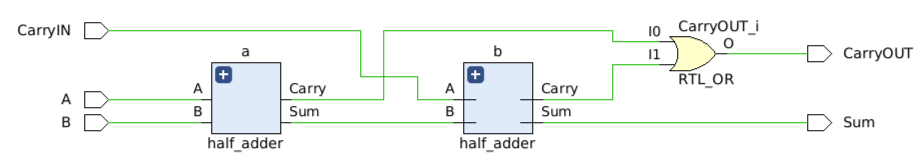
\includegraphics[width=\textwidth]{apple.png}
\subsection{2.5B)}
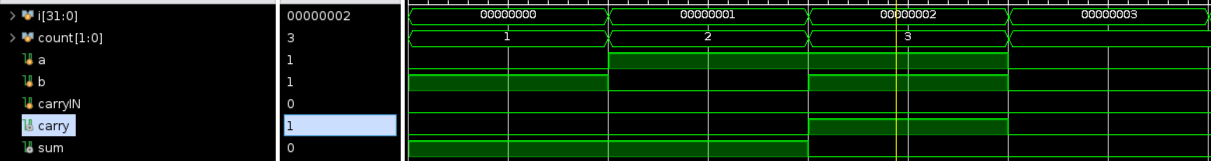
\includegraphics[width=\textwidth]{beta.png}

\pagebreak
\section{2.8}
\textbf{Given:} A firm's short-run cost function for the production of gizmos is given by the following expression: $$ C(y) = 10*y^2 + 200*y + 100,000 $$

\subsection{A) Calculate the range of output over which it would be profitable for this firm to produce gizmos if it can ell each gizmo for \$2400. Calculate the value of the output that maximizes this profit.}


\subsection{B) Repeat these calculations and explain your results fo rthe case in which the short-run cost function is given by $$ C(y) = 10*y^2 + 200*y + 200,000 $$}


\end{document}
